\chapter{Cosmology Lecture 4: Homogeneity, Friedmann Dynamics, and the Equation of State}

This is a lecture in which the questions are not a digression. They are the mechanism by which the formalism arrives. Before a single new cosmological equation is allowed onto the board, we are forced to confront several sources of confusion: could the universe be smaller than the part we observe, why do atoms and planets not simply join the general expansion, what becomes of energy conservation in a time-dependent background, and what do homogeneity and isotropy mean mathematically rather than poetically? Only after that conceptual clearing do we write the cosmological metric, ask for its dynamics, and discover that the remaining bottleneck is not geometry but the behavior of the energy density.

\section{Opening Questions About Expansion and Size}

Susskind begins by inviting questions, and the first one is topological. Could the universe be smaller than the observable universe? The example on the table is a periodically identified space, essentially toroidal, so that one would see repetitions of the same large-scale structures and, in a loose phrase, might even be seeing oneself through the back door. The point is not that such an idea is logically forbidden. The point is that it would have observational consequences. The lecture's answer is therefore empirical in tone: people have looked for periodicity in cosmological observations, and there is no evidence for it, together with some evidence against it. For that reason the lecture treats a smaller periodically repeated universe as unsupported.

The next pressure point is more immediate. The universe expands, but the solar system does not visibly swell, atoms do not fly apart, and a person holding another person's hand does not slowly drift away because of Hubble expansion. Here the lecture insists that one must separate cosmology from local binding.

\subsection{Question \& Answer}

\paragraph{Question.} How can an expanding universe coexist with stable atoms, solar systems, and with what we mean by energy conservation?

\paragraph{Answer.} Local bound systems do not simply participate in the Hubble flow. If two people are holding hands in space, the tiny cosmological tendency to separate them is overwhelmed by the ordinary forces between them. The same is true, much more strongly, for atoms bound by electromagnetism and for planets bound by gravity. One may say, at most, that an accelerated expansion would slightly perturb a bound system and make it infinitesimally larger. But that is a tiny correction, not a mechanism for tearing the system apart.

The energy question is deeper. If the background spacetime itself changes with time, then the naive static-world form of global energy conservation is no longer the right principle. The lecture makes the point in the simplest possible way: conservation of energy is tied to time-translation invariance. If the whole setup is time independent, then the same experiment performed later or earlier gives the same result, and energy conservation follows. But in an expanding universe the background is time dependent. In that situation one should not insist that the total energy in the universe stays fixed in the ordinary static sense. Rather, the lecture says, changes in energy are tied to the kinetic energy of expansion itself. That heuristic point will later reappear in a more concrete thermodynamic form.

Another question then pushes the discussion toward geometry. On what scales is the universe really homogeneous and isotropic? The answer is: certainly not on small scales. Galaxies, stars, and atoms spoil exact homogeneity. But on sufficiently large scales, averaged over many inhomogeneities, the universe appears homogeneous and isotropic. That answer is still qualitative. To go further, we need a metric statement.

\section{Homogeneity and Isotropy as Metric Statements}

The lecture now changes register. Homogeneity and isotropy are not, first of all, dynamical statements. They are statements about geometry. Einstein's equations tell us how geometry changes with time; the claim that space is homogeneous and isotropic tells us what sort of geometry we are talking about before we ask for its time evolution.

\subsection{Question \& Answer}

\paragraph{Question.} What do homogeneity and isotropy mean mathematically?

\paragraph{Answer.} A space is described by a metric. Choose coordinates \(x\) so that one point is the origin. Then make a coordinate transformation to new coordinates \(y\), so that a different point becomes the origin. In a homogeneous space one can do this in such a way that the functional form of the metric is unchanged. That is the precise statement that every point is geometrically the same as every other. Isotropy adds the statement that, around a given point, no direction is preferred.

\begin{definition}
A space is homogeneous if for any two points there exists a coordinate transformation taking one to the other while preserving the form of the metric. A space is isotropic if, in addition, the metric near a point shows no preferred direction.
\end{definition}

The flat plane gives the simplest example. In two dimensions we may write
\begin{equation}
ds^2 = dx_1^2 + dx_2^2 .
\end{equation}
Now translate the coordinates:
\begin{equation}
y_1 = x_1 + a_1,
\qquad
y_2 = x_2 + a_2 .
\end{equation}
The parameters \(a_1\) and \(a_2\) are only shifts of origin; they have nothing to do with the cosmological scale factor that will appear later. Differentiating gives \(dy_1=dx_1\) and \(dy_2=dx_2\), so the metric becomes
\begin{equation}
ds^2 = dy_1^2 + dy_2^2 .
\end{equation}
It has exactly the same form. Therefore the neighborhood of the old origin and the neighborhood of the new one are geometrically indistinguishable. That is homogeneity in the cleanest possible setting.

The sphere gives the second example. The lecture writes the unit two-sphere metric in the form
\begin{equation}
d\Omega_2^2 = dr^2 + \sin^2 r\, d\theta^2 .
\end{equation}
If we choose the south pole as origin, then \(r\) measures distance from that pole. If we rotate the sphere and choose an east pole instead, the coordinate change is unpleasant to write explicitly, but the conclusion is simple: once everything is re-expressed relative to the new pole, the metric again takes the same form. Thus every point on the sphere is the same as every other.

In two dimensions there is a useful test: a uniform geometry has the same curvature everywhere. That is not the full definition in higher dimensions, but it captures the right idea. The flat plane, the sphere, and the hyperbolic plane are the canonical homogeneous and isotropic geometries. Cosmology lifts this pattern to three spatial dimensions.

The lecture also insists that homogeneity is scale dependent. The air in a quiet room is roughly homogeneous and isotropic on large enough scales, but not on the scale of individual molecules. Likewise the universe is not homogeneous on the scale of galaxies, clusters, or smaller structures. The statement of homogeneity belongs to large-scale cosmology.

\section{Intrinsic Geometry, Embedding, and the Torus Caveat}

At this point Susskind pauses for a conceptual warning that is essential to everything that follows. When we say that space may be spherical, we do not mean that it is literally like the rubber skin of a balloon sitting in some larger ambient space. That picture is useful only as a visual crutch, and it often misleads. The geometry relevant to cosmology is intrinsic geometry: the geometry determined by measurements made within the space itself.

A one-dimensional example is the cleanest way to force the point. Suppose we have a closed one-dimensional space. We may draw it as a circle, or as a square, or as a peanut-shaped loop. But from the intrinsic point of view the drawing is not the geometry. The only thing that matters is distance measured along the line. If two such loops have the same total circumference, then intrinsically they are the same one-dimensional space.

\begin{figure}
\centering

\includegraphics[width=0.72\textwidth]{lecture_04_figure_05.png}
\caption{Round and deformed closed loops on the board. The lecture uses them to separate intrinsic geometry from the way a space is drawn in a higher-dimensional ambient space.}
\end{figure}

This is stronger than it first sounds. The lecture emphasizes that one-dimensional spaces are intrinsically flat. Any small piece of a string can be straightened without stretching it. So the fact that a curve looks bent on the page is not intrinsic curvature. It is only curvature of embedding.

\begin{remark}
For a one-dimensional space the apparent bending of a drawn curve is extrinsic, not intrinsic. Intrinsically, the geometry is characterized only by lengths along the curve and, in the closed case, by the total circumference.
\end{remark}

A minimal redraw captures the blackboard idea while stripping away accidental clutter.

\begin{figure}
\centering
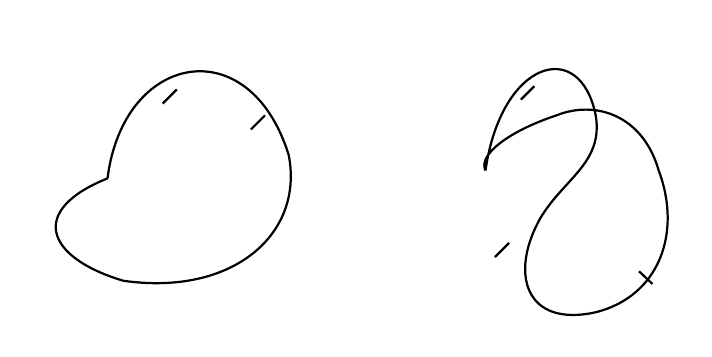
\begin{tikzpicture}[scale=1.0]
\draw[line width=0.8pt] (0,0)
  .. controls (0.2,1.6) and (1.8,1.9) .. (2.3,0.3)
  .. controls (2.5,-0.7) and (1.6,-1.5) .. (0.2,-1.3)
  .. controls (-0.8,-1.0) and (-1.0,-0.4) .. (0,0);
\draw[line width=0.8pt] (0.70,0.95) -- (0.88,1.13);
\draw[line width=0.8pt] (1.82,0.62) -- (2.00,0.80);

\draw[line width=0.8pt] (4.8,0.1)
  .. controls (5.0,1.5) and (6.0,1.8) .. (6.2,0.8)
  .. controls (6.3,0.2) and (5.8,0.0) .. (5.5,-0.5)
  .. controls (5.1,-1.2) and (5.3,-1.9) .. (6.2,-1.7)
  .. controls (7.0,-1.5) and (7.3,-0.7) .. (7.0,0.1)
  .. controls (6.8,0.8) and (6.2,1.0) .. (5.7,0.8)
  .. controls (5.1,0.6) and (4.7,0.3) .. (4.8,0.1);
\draw[line width=0.8pt] (5.25,1.00) -- (5.42,1.17);
\draw[line width=0.8pt] (5.10,-0.82) -- (4.92,-1.00);
\draw[line width=0.8pt] (6.75,-1.18) -- (6.92,-1.34);
\end{tikzpicture}
\caption{A clean redraw of the lecture's circle and peanut-shaped loop. Equal circumference means equal intrinsic one-dimensional geometry.}
\end{figure}

The lecture then generalizes the warning. A flat sheet of paper rolled into a cylinder is still intrinsically flat. Nothing about distances measured within the sheet changes merely because we bent it in the surrounding space. A hemisphere is different: it cannot be flattened without stretching, so its intrinsic geometry is curved. That is the real distinction.

This is also where the torus caveat belongs. A torus with periodic identifications is translation invariant, so in that sense it is homogeneous. But it is not isotropic. The periodic directions define preferred axes. Observations made along one of those axes are not equivalent to observations made along a generic oblique direction. Thus the torus is an example of a homogeneous space that fails to be isotropic.

The lecture even pushes the intrinsic point into an almost science-fiction picture. Imagine creatures confined to an optical fiber, able to send signals only along the fiber. For them, a straight segment and a bent segment would be indistinguishable as long as the internal distances are the same. Only if some signal escaped the fiber could they discover the larger embedding space. Cosmology, as used here, is about what can be measured within the geometry, not about the external picture we use to help ourselves visualize it.

Only now is the lecture ready to say: let us accept homogeneous and isotropic space and move on.

\section{The FRW Ansatz and the Three Curvature Cases}

Having cleared away the bad pictures, the lecture finally writes the cosmological metric. We assume that on sufficiently large scales space is homogeneous and isotropic, so at any fixed time it must be one of three geometries: positively curved, flat, or negatively curved. The names are deliberately unromantic:
\begin{equation}
k=+1,\qquad k=0,\qquad k=-1 .
\end{equation}
Here \(k\) is simply the curvature label.

The blackboard organizes the spatial possibilities under a common factor \(a(t)^2\):

\begin{figure}
\centering

\includegraphics[width=0.74\textwidth]{lecture_04_figure_02.png}
\caption{Grouped spatial metrics and curvature labels. The common multiplier \(a(t)^2\) is the scale factor.}
\end{figure}

The spacetime ansatz is
\begin{equation}
ds^2=-dt^2+a(t)^2\,d\Sigma_k^2 .
\end{equation}
The minus sign in front of \(dt^2\) is the relativistic sign convention. The important structural assumption is that, in these coordinates, space and time are not mixed. Later in the lecture this is explicitly justified as a consequence of homogeneity and isotropy: if the universe is homogeneous and isotropic and remains so, there is essentially no alternative.

The three spatial metrics are
\begin{align}
d\Sigma_{0}^{2} &= dx^{2}+dy^{2}+dz^{2}
               = dr^{2}+r^{2}d\Omega_{2}^{2}, \\
d\Sigma_{+1}^{2} &= d\Omega_{3}^{2}
                 = dr^{2}+\sin^{2}r\,d\Omega_{2}^{2}, \\
d\Sigma_{-1}^{2} &= dr^{2}+\sinh^{2}r\,d\Omega_{2}^{2}.
\end{align}
At any fixed time the spatial universe is therefore either flat, spherical, or hyperbolic. What changes with time is the overall scale \(a(t)\).

Now the lecture extracts Hubble's law purely kinematically. Fix two galaxies at fixed comoving coordinates. Their coordinate separation does not change, but their physical distance does. If \(\Delta\chi\) denotes the fixed coordinate separation, then
\begin{equation}
D(t)=a(t)\,\Delta\chi .
\end{equation}
Differentiate with respect to time:
\begin{equation}
v(t)=\dot a(t)\,\Delta\chi .
\end{equation}
Eliminate \(\Delta\chi\), and we get
\begin{equation}
v=\frac{\dot a}{a}\,D .
\end{equation}
This is Hubble's law. The quantity \(\dot a/a\) need not be constant in time, but it does not depend on position. That is the sense in which the Hubble parameter is universal in the homogeneous model.

The lecture also pauses over the meaning of \(a(t)\). In the \(k=+1\) case its interpretation is especially clean: it is the radius of the spatial three-sphere. In the flat case, where the universe is infinite, \(a(t)\) by itself has no invariant absolute meaning. Only ratios of scale factors or physical distances matter. In the negatively curved case there is again a natural hyperbolic radius. This distinction matters because it warns us not to assign too concrete a picture to \(a(t)\) in the flat case.

\section{From Einstein's Equation to Friedmann}

Once the metric is on the board, kinematics is exhausted. The next move is explicit: now what do we do with it? We want equations for \(a(t)\). Since the metric is curved, we are no longer allowed to begin with Newtonian mechanics as the starting point. We must use general relativity, even though the final cosmological equation will turn out to be the same equation we already met in Newtonian form.

Susskind is equally explicit about what he is not going to do. He is not going to compute all the Christoffel symbols on the board. That is a nuisance, and it is not the conceptual point of the lecture. Instead he writes the general structure of Einstein's equation and then extracts the one component needed for this symmetric cosmology.

\begin{figure}
\centering

\includegraphics[width=0.78\textwidth]{lecture_04_figure_03.png}
\caption{Einstein equation as written on the board. The visible frame clearly shows the geometric left-hand side and the prefactor \(8\pi G/3\).}
\end{figure}

For the cosmological reduction discussed in the lecture we write
\begin{equation}
R^{\mu\nu}-\frac{1}{2}g^{\mu\nu}R=\frac{8\pi G}{3}\,T^{\mu\nu}.
\end{equation}

\begin{remark}
The board visibly shows the geometric left-hand side together with the prefactor \(8\pi G/3\). The tensor \(T^{\mu\nu}\) is supplied by the transcript. This normalization is lecture-faithful for the cosmological discussion, even though it is not the standard way one usually displays the full Einstein equation in textbook tensor notation.
\end{remark}

The right-hand side is matter: the energy-momentum tensor. It contains energy density, momentum density, and fluxes. For the homogeneous cosmology under discussion we focus on the time-time component, because
\begin{equation}
T_{00}=\rho .
\end{equation}
So the right-hand side becomes the energy density of the material filling the universe.

The left-hand side is geometry. The lecture emphasizes two structural facts about its time-time component. First, the Einstein-tensor combination is special: the terms containing second derivatives of the metric cancel in the time-time component. What survives is quadratic in first derivatives. Second, the surviving terms separate into a time-evolution piece and a purely spatial-curvature piece. The time-evolution piece is proportional to \(\dot a^{2}/a^{2}\); the spatial-curvature piece is proportional to \(k/a^{2}\).

This is enough to land on the Friedmann equation in the lecture-aligned form
\begin{equation}
\left(\frac{\dot a}{a}\right)^{2}+\frac{k}{a^{2}}=\frac{8\pi G}{3}\rho .
\end{equation}
The lecture then moves the curvature term to the other side and writes
\begin{equation}
\left(\frac{\dot a}{a}\right)^{2}=\frac{8\pi G}{3}\rho-\frac{k}{a^{2}} .
\end{equation}

\subsection{Question \& Answer}

\paragraph{Question.} Why is the time-time component enough, and where did the second derivatives go?

\paragraph{Answer.} In the homogeneous and isotropic ansatz there is only one unknown function, \(a(t)\). Because there is only one function to determine, one nontrivial Einstein equation is enough. The mixed space-time components give only \(0=0\) in this ansatz. The space-space components are equivalent to the time-time component, or to linear combinations of it, and one can choose combinations that look more like the Newtonian \(F=ma\) equation and contain \(\ddot a\). But the time-time component is especially convenient because in that component the second-derivative terms cancel inside the Einstein tensor, leaving the cosmological energy equation above.

This is the point at which the lecture makes its most striking comparison with the Newtonian analysis. The equation is exactly the same differential equation we already studied there. The novelty is not the form of the equation but the interpretation of the curvature term. In the Newtonian story the corresponding constant had to do with total energy and escape velocity. Here the same slot is occupied by the intrinsic curvature of space. The mathematics is the same; the physical meaning has shifted.

The lecture also explains why that coincidence is not mysterious. If we look at a sufficiently small patch of a curved universe, the curvature is negligible, and local dynamics must reduce to the Newtonian picture. Once one sees that the same equation governs both the small patch and the homogeneous whole, one should expect the Newtonian form to reappear.

There is one more beat before moving on. With only matter and radiation present, the sign of \(k\) is correlated with the future history of the universe: positive curvature corresponds to recollapse, negative curvature to continued expansion, and \(k=0\) to the knife-edge case. But the lecture immediately warns us not to take that as a universal truth. Dark energy will spoil this simple correlation.

\section{Equation of State and Density Scaling}

At this stage the lecture has an equation for \(a(t)\), but it is not yet usable. There is not much one can do with Friedmann's equation unless one knows how \(\rho\) depends on the scale factor. Susskind says this very plainly. The remaining unknown is not geometric; it is material. We need to know how different kinds of stuff dilute, or fail to dilute, as the universe expands.

Before going general, the lecture recalls the two examples already familiar from earlier discussions:
\begin{equation}
\rho_{\text{matter}}=\frac{\rho_{0}}{a^{3}},
\qquad
\rho_{\text{rad}}=\frac{\rho_{0}}{a^{4}}.
\end{equation}
The board then reframes these examples through a single thermodynamic idea.

\begin{figure}
\centering

\includegraphics[width=0.82\textwidth]{lecture_04_figure_06.png}
\caption{Equation of state with matter and radiation scalings. The board stages the transition from specific examples to the general relation \(P=w\rho\).}
\end{figure}

The organizing principle is the equation of state,
\begin{equation}
P=w\rho .
\end{equation}
On the board the parameter is written as an uppercase \(W\); in the notes we normalize it to \(w\). The lecture explicitly says that the strategy now has two steps. First, assume an equation of state and derive how \(\rho\) scales with \(a\). Second, in the next lecture, derive \(w\) for different kinds of material. For the present lecture only the first step is carried out.

\begin{definition}
An equation of state is a relation between thermodynamic variables. In the present setting it is the relation between pressure \(P\) and energy density \(\rho\), taken in the form \(P=w\rho\).
\end{definition}

The familiar cases fit into this scheme. Matter domination means particles moving slowly with negligible pressure, so
\begin{equation}
w=0 .
\end{equation}
Radiation domination means
\begin{equation}
w=\frac13 .
\end{equation}
The lecture notes that the factor \(1/3\) comes from three spatial dimensions, although its derivation is deferred.

Now comes the thermodynamic derivation. Consider a box of material with volume \(V\), energy density \(\rho\), and total energy
\begin{equation}
E=\rho V .
\end{equation}
For a slow adiabatic change, the only thermodynamic identity we need is
\begin{equation}
dE=-P\,dV .
\end{equation}
The sign matters: if the box expands, the system does work on the walls, so the energy in the box decreases. On the other hand,
\begin{equation}
dE=\rho\,dV+V\,d\rho .
\end{equation}
Equating the two expressions for \(dE\) gives
\begin{align}
\rho\,dV+V\,d\rho &= -P\,dV, \\
V\,d\rho &= -(\rho+P)\,dV .
\end{align}
Now insert the equation of state \(P=w\rho\):
\begin{equation}
V\,d\rho=-(1+w)\rho\,dV .
\end{equation}
Divide by \(\rho V\):
\begin{equation}
\frac{d\rho}{\rho}=-(1+w)\frac{dV}{V} .
\end{equation}
Both sides are logarithmic differentials,
\begin{equation}
d(\log\rho)=-(1+w)\,d(\log V) ,
\end{equation}
so integration yields
\begin{equation}
\rho\propto V^{-(1+w)} .
\end{equation}
For a comoving box expanding with the universe,
\begin{equation}
V\propto a^{3} .
\end{equation}
Therefore
\begin{equation}
\rho\propto a^{-3(1+w)},
\end{equation}
or, with the integration constant written explicitly,
\begin{equation}
\rho=\frac{\text{const.}}{a^{3(1+w)}} .
\end{equation}

Now the earlier examples reappear automatically:
\begin{align}
w=0 &\Longrightarrow \rho\propto a^{-3}, \\
w=\frac13 &\Longrightarrow \rho\propto a^{-4}.
\end{align}
This is exactly the lecture's point. Matter domination and radiation domination are not isolated facts; they sit inside a more general framework.

It is useful, and faithful to the lecture, to connect this back to the old flat-universe solutions. For \(k=0\), the Friedmann equation becomes
\begin{equation}
\left(\frac{\dot a}{a}\right)^{2}=\frac{8\pi G}{3}\rho .
\end{equation}
In a matter-dominated universe,
\begin{equation}
\rho=\frac{\rho_{0}}{a^{3}},
\end{equation}
so
\begin{equation}
\dot a^{2}\propto \frac{1}{a}.
\end{equation}
Integrating,
\begin{equation}
a(t)\propto t^{2/3}.
\end{equation}
In a radiation-dominated universe,
\begin{equation}
\rho=\frac{\rho_{0}}{a^{4}},
\end{equation}
so
\begin{equation}
\dot a^{2}\propto \frac{1}{a^{2}},
\end{equation}
and hence
\begin{equation}
a(t)\propto t^{1/2}.
\end{equation}
These are exactly the results obtained in the earlier Newtonian treatment. Again, the lecture pauses to reassure the audience: that earlier work was not wasted.

At the end Susskind deliberately opens the door to a new case. Vacuum energy, dark energy, and the cosmological constant are all identified here with
\begin{equation}
w=-1 .
\end{equation}
The lecture notes how odd this looks: pressure and energy density have opposite signs. Negative pressure is tension rather than compression. As a simple intuition pump, one may think of a stretched spring, which pulls inward rather than pushing outward. The lecture does not claim that a spring is a model of dark energy; it uses the example only to make negative pressure less alien.

Once \(w=-1\) is inserted into the scaling law, the result is immediate:
\begin{equation}
\rho\propto a^{0}=\text{constant}.
\end{equation}
That is the character of vacuum energy. Expanding the box changes the total energy in the box, but it does not dilute the energy density. Empty space keeps the same energy density when stretched.

The lecture stops here on purpose. It briefly remarks that the radiation today is overwhelmingly the cosmic microwave background and is a very small fraction of the total cosmic energy budget, while running backward in time makes radiation dominate the early universe. But the real dynamics of the \(w=-1\) case are deferred. This lecture wants only to put the new ingredient on the table and leave its consequences for the next step.

\section{Summary}

The lecture begins by using questions to expose the conceptual obstacles that cosmology creates. A periodically identified small universe would produce repeated images. Bound systems do not simply follow the cosmological expansion because local binding forces overwhelm the tiny expansive tendency. And the ordinary static-world notion of global energy conservation cannot be carried unchanged into a time-dependent background.

From there the lecture turns those questions into geometry. Homogeneity and isotropy are statements about the form of the metric. They are scale-dependent statements, and they must be understood intrinsically rather than through misleading embedding pictures. The long discussion of circles, peanut-shaped loops, cylinders, and spheres is not ornamental; it is what makes the later cosmological metric intelligible.

Once that groundwork is done, the cosmological ansatz
\begin{equation}
ds^{2}=-dt^{2}+a(t)^{2}d\Sigma_{k}^{2}
\end{equation}
arrives naturally, together with the three spatial curvature cases and the purely kinematic derivation of Hubble's law,
\begin{equation}
v=\frac{\dot a}{a}D .
\end{equation}
General relativity then supplies the dynamics. In the time-time component of Einstein's equation the second-derivative terms cancel, and one obtains the Friedmann equation
\begin{equation}
\left(\frac{\dot a}{a}\right)^{2}=\frac{8\pi G}{3}\rho-\frac{k}{a^{2}} .
\end{equation}
Its form is the same as in the Newtonian treatment, but the curvature term now carries the intrinsic geometry of space.

Finally, the lecture identifies the remaining missing input: how \(\rho\) changes as the universe expands. The equation of state \(P=w\rho\), together with the adiabatic identity \(dE=-P\,dV\), yields
\begin{equation}
\rho\propto a^{-3(1+w)} .
\end{equation}
Matter and radiation reappear as \(w=0\) and \(w=\tfrac13\), and the lecture closes by placing \(w=-1\) on the board as the signature of vacuum energy. That is the point at which this chapter stops: the framework is in place, and dark energy has appeared, but its full consequences are left for the next lecture.